\documentclass[alg,german,seminar,pdf,article]{unitext}

\usepackage[utf8]{inputenc}

\usepackage{enumitem}
\makeatletter
\let\mdwNote\note                        % make \IEEEproof do same as \proof
\let\note\@undefined                        % undefine \proof
\makeatother

\usepackage{calligra}
\usepackage{amsmath}
\usepackage{amsthm}
\usepackage{stmaryrd}

%\usepackage{algorithmic}
%\usepackage{algorithm}
%\numberwithin{algorithm}{chapter}
%\usepackage{gnuplottex}

\usepackage{tikz}
\usepackage{environ}
\makeatletter
\newsavebox{\measure@tikzpicture}
\NewEnviron{scaletikzpicturetowidth}[1]{%
  \def\tikz@width{#1}%
  \def\tikzscale{1}\begin{lrbox}{\measure@tikzpicture}%
  \BODY
  \end{lrbox}%
  \pgfmathparse{#1/\wd\measure@tikzpicture}%
  \edef\tikzscale{\pgfmathresult}%
  \BODY
}
\makeatother

\usepackage[final]{pdfpages}
%\usepackage[draft]{pdfpages}

\newtheoremstyle{note} % name
                {10pt} %Space above               
                {10pt} %Space below
                {\itshape} %Body font
                {} %Indent amount
                {\bfseries} % Theorem head font
                {:} %Punctuation after theorem head
                {.5em} %Space after theorem head
                {} %Theorem head spec (can be left empty, meaning ‘normal’)

\newtheoremstyle{definition} % name
                {10pt} %Space above               
                {10pt} %Space below
                {} %Body font
                {} %Indent amount
                {\bfseries} % Theorem head font
                {} %Punctuation after theorem head
                {\newline} %Space after theorem head
                {} %Theorem head spec (can be left empty, meaning ‘normal’)

\newtheoremstyle{theorem} % name
                {10pt} %Space above               
                {10pt} %Space below
                {\itshape} %Body font
                {} %Indent amount
                {\bfseries} % Theorem head font
                {} %Punctuation after theorem head
                {.5em} %Normal Space after theorem head
                {} %Theorem head spec (can be left empty, meaning ‘normal’)

\newtheoremstyle{example} % name
                {10pt} %Space above               
                {10pt} %Space below
                {} %Body font
                {} %Indent amount
                {\bfseries} % Theorem head font
                {} %Punctuation after theorem head
                {\newline} %Space after theorem head
                {} %Theorem head spec (can be left empty, meaning ‘normal’)


\theoremstyle{definition}
%\newtheorem{definition}{Definition}[chapter]
\newtheorem{definition}{Definition}[section]

\theoremstyle{theorem}
\newtheorem{theorem}[definition]{Satz}
\newtheorem{lemma}[definition]{Lemma}
\newtheorem{corollary}[definition]{Korollar}
\newtheorem{problem}[definition]{Problem}

\theoremstyle{example}
\newtheorem{example}[definition]{Beispiel}

\theoremstyle{remark}
\newtheorem{remark}[definition]{Bemerkung}

\renewcommand{\proofname}{Beweis}

%%% named references
\newcommand{\refRemark}[1]{Remark \ref{#1}}
\newcommand{\theoRef}[1]{Theorem \ref{theo:#1}}
\newcommand{\corRef}[1]{Corollary \ref{cor:#1}}
\newcommand{\lemRef}[1]{Lemma \ref{lem:#1}}
\newcommand{\probRef}[1]{Problem \ref{prob:#1}}

%%% Highlighting and indexing of terms
\newcommand{\term}[1]{\emph{#1}\index{#1}}

% reduce space around cdot
\let\oldcdot=\cdot
\def\cdot{\negthinspace\oldcdot\negthinspace}

\def\notmid{\!\!\:\!\not|\;}

\newcommand{\R}{\mathbb{R}}
\newcommand{\Rd}{\R^d}
\newcommand{\Sd}[1]{\mathbb{S}_{#1}}
\newcommand{\Bd}{\mathbb{B}_{d}}
\newcommand{\I}{[0,1]}
\newcommand{\RdEx}{\widehat{\mathbb{R}}^d}

%% Möbius groups
\DeclareMathOperator{\GM}{GM}
\newcommand{\GMRd}{\GM(\Rd)}
\DeclareMathOperator{\M}{M}
\newcommand{\MRd}{\M(\Rd)}
\newcommand{\MSd}{\M(\Sd{d-1})}

%% Operators %%
\DeclareMathOperator{\grad}{grad}
\DeclareMathOperator{\im}{im}
\DeclareMathOperator{\Conf}{Conf}

%% sets of differentiable functions %%
\newcommand{\diffPw}[3]{C^{#1}_{\mathcal{P}}({#2}, {#3})}
\newcommand{\diffRdPw}[2]{\diffPw{#1}{#2}{\Rd}}
\newcommand{\diffRd}[2]{C^{#1}({#2}, \Rd)}
\newcommand{\diff}[3]{C^{#1}({#2}, {#3})}

%% Special functions/operators
\newcommand{\arclength}[1]{\ell({#1}, \mathcal{P})}
\newcommand{\norm}[1]{\left\Vert{#1}\right\Vert}
\newcommand{\inner}[2]{\left\langle{#1},{#2}\right\rangle}

%% Set definitions
\newcommand{\where}{\:|\:} % for set definitions
\newcommand{\setDef}[2]{\left\{{#1} \:|\: {#2}\right\}}


%%%%%%%% textual formatings %%%%%%%%%%
\newcommand{\resp}{\mbox{resp.}\ }
\newcommand{\st}{\mbox{s.t.}\ }


\graphicspath{{images/}}

\title{Snake Charmer's Problem}
\author{Henning Basold}
\date{October 17th, 2011}
\dozent{Dr. Iris Reinbacher}
%\betreuer{Matthias Hanke}

\renewcommand{\purposename}{Purpose}
\renewcommand{\abstractname}{Abstract}

%\keywords{Elliptic Curve Cryptography, Parallelization, Key Agreement}
%\makeglossary
%\makeindex
%\makenomenclature

\begin{document}

%\titelblatt             %%% obligatorisch
%\zusammenfassung        %%% obligatorisch, in der Datei abstract.tex
%\cleardoublepage
%\tableofcontents        %%% obligatorisch
%\listoftables           %%% optional
%\listoffigures          %%% optional
%\abkuerzung             %%% optional, in der Datei abbreviation.tex

\starttext
%\chapter{Mathematical Foundations}\label{chap:math}

\section{Problem description}\label{sec:problem}
The problem that will be tackled in this talk is called the ”Snake Charmer's Problem”.
It is about deforming a curve (the \emph{snake}) \st its \emph{snout} follows another
given curve (the snake charmer).

More precisely: a curve $S : [0,L] \rightarrow \Rd$ of length $L$ which is
piece-wise differentiable, has arc-length $L$ and fixed \term{tail} $S(0) = 0$ is called
a \term{snake}. $S(L)$ is called the \term{snout}.

Given a snake and a continuously differentiable curve $\gamma : [0,1] \rightarrow \Rd$.
Find a family $S_t, t \in [0,1]$ of snakes of length $L$ \st $S_0 = S$ and its
snouts follow $\gamma$: $S_t(L) = \gamma(t)$.

In the following the necessary definitions will be given to understand the above
description fully and to be able to reformulate the problem into a solvable
problem.

Everything will be formulated in a way that the topic is understandable without
having deep knowledge about Topology, manifolds and so on. Only a geometric imagination
of spheres, planes and curves in $\Rd$ (mostly $\R^3$) is needed. The purpose of this
report and talk is to demonstrate the power of topological abstraction in solving
problems coming from computer science.


\section{Configuration space}\label{sec:conf}
%\begin{definition}[Topology]
%    Let $X$ be a set. If $\mathcal{O} \subseteq 2^X$ satisfies
%    \begin{enumerate}
%        \item $\forall \{U_{\alpha} | \alpha \in A\} \subseteq \mathcal{O}:
%                   \cup_\alpha U_\alpha \in \mathcal{O} $ 
%        \item $\forall U,V \in \mathcal{O}: U \cap V \in \mathcal{O}$
%        \item $\emptyset, X \in \mathcal{O}$
%    \end{enumerate}
%    then $\mathcal{O}$ is called a \term{topology} on $X$ and $X$ is called a
%    \term{topological space}. A set $U \in \mathcal{O}$ is called \term{open}.
%\end{definition}
%
%\begin{definition}[Continuous]
%    Let $X,Y$ be topological spaces and $f : X \rightarrow Y$ be a map.
%    If $f^{\leftarrow}(U) = \{x \in X | f(x) \in U \}$ is open in $X$, than
%    $f$ is called \term{continuous}.
%\end{definition}

%\begin{definition}[Piecewise differentiable]
%    Let $f : [0,L] \rightarrow \Rd, L \in \R_{>0}$ be a function and
%    $\mathcal{P} = \{0 = s_0 < s_1 < \ldots s_{N-1}, s_N = L\}$ a partition of $[0,L]$.
%    If all derivatives \[ \cfrac{d^j f_i}{d x^j} \]
%    exists and are continuous on for $j=0, \ldots, k$ and
%    $f(x) = (f_1(x), \ldots, f_d(x))$
%    then $f$ is called \term{k-times piecewise differentiable}. The class of all those
%    functions is denoted as $\diffRdPw{k}{[0,L]}$.
%\end{definition}

The class of all \term{k-times continuously differentiable} functions from
$[a,b] \subseteq \R$ to $\Rd$ is denoted as $\diffRd{k}{[a,b]}$. We refine this
class in the following sense:

\begin{definition}[Piecewise differentiable]
    Let $f : [0,L] \rightarrow \Rd, L \in \R_{>0}$ be a function. If there exists a
    partition $\mathcal{P} = \{0 = s_0 < s_1 < \ldots s_{N-1}, s_N = L\}$ of $[0,L]$
    \st $f_i = f|_{[s_i,s_{i+1}[} \in \diffRd{k}{[s_i,s_{i+1}[}$
    for all $i=0, \ldots, N-1$ and
    $f_i$ can be continuously extended to a map from $[s_i,s_{i+1}]$ to $\Rd$
    then $f$ is called \term{k-times piecewise continuously differentiable}.
    
    The class of all those functions is denoted by $\diffRdPw{k}{[0,L]}$.
\end{definition}

\begin{remark}
    As functions from $\diffRd{k}{[a,b]}$ have to be continuously differentiable
    $\diffRd{0}{[a,b]}$ denotes all continuous functions from $[a,b]$ to $\Rd$.
\end{remark}

To make clear what the length of snake means, we make the following definition:
\begin{definition}[Euclidean arc length]
    Let $\gamma \in \diffRdPw{1}{[0,L]}$. Then its (Euclidean) \term{arc length}
    is given by
    \[
        \arclength{\gamma}
        = \sum_{i=0}^{N-1}\int_{s_i}^{s_{i+1}} |\gamma'(t)| dt
    \]
    See \cite[p. 31]{Ratcliff}.
\end{definition}

With these definitions we can describe the snake charmer's problem more precisely:
\begin{definition}
    A \term{snake} is a map $S \in \diffRdPw{1}{[0,L]}, L \in \R_{>0}$
    with arc length $L$ which is rooted at the origin: $S(0) = 0$.
    
    So its derivatives exist everywhere except at $s_1, \ldots, s_{N-1}$ where
    they are extended by
    \[
        \left.\frac{dS}{ds}\right|_{s_i} = \lim_{s \downarrow s_i}\frac{dS}{ds}(s).
    \]
    
    $\lim_{s \downarrow s_i}$ denotes the limit of a function if s get arbitrary
    close to $s_i$ coming from values greater than $s_i$.

    $S(L)$ is called the \term{snout} of the snake.
\end{definition}

\begin{lemma}
    Observe that since $\arclength{S} = L$ it follows that
    \[
        \norm{\frac{dS}{ds}(\sigma)} = 1 \text{ for all } \sigma \in [0,L] .
    \]
    
    So it follows
    \[  \frac{dS}{ds}([0,L]) \subseteq \Sd{d-1} . \]
    See \cite[p. 35-36]{Tarapov} and \cite{Rodriguez07}.
\end{lemma}

With this we can define the configuration space of the snakes:
\begin{definition}[Configuration space]
    \[\Conf_{\mathcal{P}}(d-1) = \diffPw{0}{[0,L]}{\Sd{d-1}} \]
    is the \term{configuration space} of snakes of length $L$.
    It will be abbreviated as $\Conf$ in the following.
    Points $z \in \Conf$ are called \term{configurations}.
\end{definition}

\begin{remark}
    Observe that we can reconstruct a unique snake from a configuration $z$,
    since the tail is fixed:
    \[
        S_z(s) = \int_0^s z(\sigma) d\sigma
    \]
\end{remark}

With this we define the following for the rest of this text:
\begin{definition}
    \[f : \Conf \rightarrow \Rd, z \mapsto S_z(L)\]
\end{definition}

The image of $f$ is the set of all reachable points by all snakes of
length $L$ which is obviously a closed ball $L\Bd$ of size $L$:
\[
    L\Bd = \setDef{x \in \Rd}{\norm{x} \leq L}
\]

Now we can reformulate the problem:
\begin{problem}\label{prob:pathLift}
    Given an initial configuration $z \in \Conf$ and a curve
    $\gamma \in \diffRd{1}{[0,1]}$ with
    $\gamma(0) = f(z)$. Find a family of configurations $z_t$ \st $z_0 = z$ and
    $f(z_t) = \gamma(t)$.
\end{problem}

\begin{remark}\label{rem:path_lift}
    Because we are looking for a path
    $\widetilde{\gamma} : [0,1] \rightarrow \Conf, t \mapsto z_t$
    in the configuration space with $f \circ \widetilde{\gamma} = \gamma$ this
    is called a \term{path lifting problem}. See the following commutative diagram.

    \begin{center}
    \begin{tikzpicture}[node distance=3cm, auto]
      \node (I) {$[0,1]$};
      \node (Rd) [right of=I] {$\Rd$};
      \node (C) [above of=Rd] {$\Conf$};
      \draw[->] (C) to node {$f$} (Rd);
      \draw[->, dashed] (I) to node {$\widetilde{\gamma}$} (C);
      \draw[->] (I) to node [swap] {$\gamma$} (Rd);
    \end{tikzpicture}
    \end{center}
\end{remark}


\section{Solution description}\label{sec:descr}
The next step is to find a description of the solution of \probRef{pathLift}
which in turn can be used to calculate it. Observe that want to continuously
deform a configuration and so need a construction to describe derivatives
of maps into $\Conf$. This leads to tangent spaces.

\subsection{Tangent spaces, derivatives and distributions}
The idea of the \term{tangent space} is essential for the rest of this discussion.
So we will build it up in two stages: first a geometric definition and then
the transfer to a more general setting.

\begin{definition}[Geometric tangent space]
    Let $M \subseteq \Rd$ be an n-dimensional manifold where $n \leq d$.
    The \term{geometric tangent space} at $p \in M$ is defined as
        \[ T_pM = \{p\} \times \R^n . \]
\end{definition}

\begin{remark}
    Elements of $\R^n$ should be viewed as vectors which have a direction
    length. A copy of $\R^n$ is then attached as a plane perpendicular to
    $p$ at $M$.
\end{remark}

We will not use the following definition but it is a starting point if one wants
work more on these topics. For a good introduction see \cite[Chapter 3]{JLee}
and \cite[Section 5B]{Kuehnel}.

\begin{definition}[Algebraic tangent space]
    Let $M$ be a smooth manifold. A linear map $X : \diff{1}{M}{\R} \rightarrow \R$
    is called a (directional) \term{derivation} or \term{tangent vector} at $p \in M$ if
        \[ X(fg) = f(p)Xg + g(p)Xf \]
    (chain rule). Set set of all those maps is $T_pM$ the \term{tangent space}
    at $p$. $TM$ denotes the disjoint union $\bigcup_{p \in M} \{p\} \times T_pM$.
\end{definition}

Here we define the tangent space for $\Conf$ as
    \[ T_z\Conf
        = \setDef{v \in \diffRdPw{0}{[0,L]}}
            {\inner{v(s)}{z(s)} = 0 \text{ for all } s \in [0,L]}.
    \]
It will be equipped with the induced inner product
    \[ \inner{v}{w} = \int_0^L \inner{v(s)}{w(s)} ds . \]

Obviously there are many more deformations of configuration possible than we need to
achieve our goal to let the snout follow a curve. We are only interested in those
deformations that require minimal ”energy” to let the snout go into a given direction.
So we only look at subsets of the tangent space $T_z\Conf$. This is where distributions
come into play (\cite[p. 8]{Rodriguez06}).

Informally a \term{distribution} or \term{generalized functions} defines
something like a derivative. Suppose we have a continuous function
$\varphi : \I \rightarrow M$ which is not everywhere differentiable,
so $\dot{\varphi}$ does not exist everywhere. Then we can relax this
to a generalized function which is not everywhere defined.
See \cite[p. 228ff]{EncyplopMath} and \cite[p. 257]{Treves}.
The definition of a distribution in a general setting is much more involved,
but is not needed for a geometric understanding. Good texts about distributions
are \cite[p. 158]{Boothby}, \cite[p. 34]{Chern} and \cite[p. 86ff]{Chevalley}.

Let us define a distribution for our problem:
\begin{definition}
    Let $\Delta_z \subseteq T_z\Conf$ be the set of all deformations $v$ of $z$
    where $\norm{v}$ is minimal when follwing a given direction $x \in T_{f(z)}\Rd$.
    The collection of all those $\Delta_z$ is denoted as $\Delta$.
\end{definition}

Since we are looking for a subset of all all those movements, we can refine the
path lifting from \refRemark{rem:path_lift}:
\begin{definition}[Horizontal]
    Let $\delta : \I \rightarrow \Conf$ be a $C^1$ curve. If
    $\dot{\delta}(t) \in \Delta_{\delta(t)}$ then $\delta$
    is called \term{horizontal}.
    
    Let $\gamma : \I \rightarrow \Rd$ be a $C^1$ curve.
    $\widetilde{\gamma} : [0,1] \rightarrow \Conf$ is called
    a \term{horizontal lift} if it is horizontal and
    $f \circ \widetilde{\gamma} = \gamma$.
\end{definition}

So we will study the following set:
\begin{definition}
    The \term{accessibility set} for a configuration $z \in \Conf$ is
    given by
    \[ \mathcal{A}(z) =
        \setDef{\gamma(1) \in \Conf}{\gamma : \I \rightarrow \Conf
            \text{ is horizontal and } \gamma(0) = z}.
    \]
\end{definition}

Before we go an we will formalize the distribution $\Delta$. For this we
need a map to go from the tangent space of the configurations to
the tangent space of the snout.

The following definition is again only given for better orientation in the literature.
\begin{definition}
    Let $M$ and $N$ be smooth manifolds and $F : M \rightarrow N$ a smooth map.
    For each $p \in M$ we define a map $T_pF : T_pM \rightarrow T_{F(p)}N$ by
        \[ (T_pFX)(g) = X(g \circ F) . \]
    It is called \term{tangent map} or \term{pushforward}.

    It satisfies the chain rule:
        \[ (T_pFX)(hg) = h(F(p))(T_pFX)(g) + g(F(p))(T_pFX)(h) . \]
\end{definition}

The geometric interpretation is as follows: if we follow $v$ in $T_zF(v)$, how
does the image of $F$ change. So the pushforward here is the Jacobian matrix,
the matrix of all partial derivatives. An exact geometric definition can
be found in \cite[Section 5B]{Kuehnel} and a good explanation in \cite[Chapter 3]{JLee}.

If we transfer this to $f : \Conf \rightarrow \Rd$ then
$T_zf : T_z\Conf \rightarrow T_{f(z)}\Rd = \Rd$ can be interpreted as: we take $z$
and deform it by $v \in T_z\Conf$, how does the snout move?
In a more computable manner:
    \[ T_zf(v) = \int_0^L v(s) ds .\]
    
So when does the snout \emph{not} move? For this recall the kernel of a function:
\begin{definition}
    Let $g : A \rightarrow B$ be a map between vector spaces. The \term{kernel}
    of $g$ is the set of all vector that are send to zero:
    \[ \ker g = \setDef{x \in A}{g(x) = 0} \]
\end{definition}

So $\ker T_zf$ is the set of all configuration changes where the snout does not move.
How does this help us to describe $\Delta$? Consider the orthogonal complement:
\begin{definition}
    Let $W$ be a space with an inner product. To vectors $x,y \in W$ are
    called \term{orthogonal} if $\inner{x}{y} = 0$.
    
    Let $U \subseteq W$. Then the \term{orthogonal complement} of $U$ is
    the set of vectors that are orthogonal to all vectors in $U$:
    \[U ^{\perp} = \setDef{y \in W}{\forall x \in U: \inner{x}{y} = 0} \]
    (see \cite[§62]{Halmos})
\end{definition}
% more infos: https://secure.wikimedia.org/wikipedia/en/wiki/Orthogonal_complement

\begin{definition}[Direct sum]
    Let $U$ and $V$ be vector spaces. The \term{direct sum}
    $W = U \oplus V$ is the Cartesian product $U \times V$
    with the induced operation
    \[ \alpha_1 (x_1,y_1) + \alpha_2 (x_2,y_2)
        = (\alpha_1 x_1 + \alpha_2 x_2, \alpha_1 y_1 + \alpha_2 y_2) \]
    (see \cite[§18]{Halmos})
\end{definition}

\begin{theorem}
    If $M$ is a subspace of $W$ of finite (co)dimension where $W$ has an
    inner product, then
    \[ W = M \oplus M^{\perp} \]
    
    See \cite[§66]{Halmos}, \cite[p.22]{Rodriguez07} and \cite[p.121]{Treves}.
\end{theorem}

% Example: R^2 = R_x \oplus R_y, x-/y-axis
% see: https://secure.wikimedia.org/wikipedia/en/wiki/Direct_sum#Internal_direct_sum

With this we can decompose $T_z\Conf$ into
    \[ T_z\Conf = \ker T_zf \oplus (\ker T_zf)^{\perp} .\]
Since $\ker T_zf$ means that the snout does not move, $\Delta_z = (\ker T_zf)^{\perp}$
achieves what we wanted.

% for later use:
%    If $f$ is differentiable for all $k \in \N$, then this class is denoted as
%    $\diffRd{\infty}{[0,L]}$ and f is called \term{smooth}.


\subsection{Möbius Transformations and the Möbius Group}
We are now going to discuss Möbius transformations which we will be using to to
describe the accessibility set. We will only discuss them in $\Rd$ but that should
be enough to build up some intuition to transfer it to $\Sd{d-1}$ where it will be
needed. The following is depicted from \cite[p. 20ff]{Beardon}.

Consider the sphere with center $a \in \Rd$ and radius $r > 0$ in $\Rd$
    \[ S(a,r) = \setDef{x \in \Rd}{\norm{x - a} = r} . \]
Let us define a \term{reflection} $\phi : \Rd \rightarrow \Rd$ at such a sphere.
In the case of the unit sphere $\Sd{d-1} = S(0,1)$ this is easily done by
    \[ \phi(x) = x/\norm{x}^2 . \]
That is norming $x$ to one and then pushing it out or pulling it in \resp by its
reciprocal length. Let us denote that operation by $x^* = x/\norm{x}^2$.
Using this notation the reflection can be easily extended to arbitrary spheres:
    \[ \phi(x) = a + r^2(x - a)^* . \]
Observe that this is not defined when $x = a$. This is overcome by extending
the space by an extra point which is not in $\Rd$
    \[ \RdEx = \Rd \cup \{\infty\} \]
and setting $\phi(a) = \infty$ since $\norm{\phi(x)} \rightarrow \infty$ when
$x \rightarrow a$. For the same reason we set $\phi(\infty) = a$.

Obviously $\phi : \RdEx \rightarrow \RdEx$ is now bijective and $\phi^2(x) = x$,
so it is its own inverse. Furthermore $\phi(x) = x$ iff $x \in S(a,r)$.

Another \term{reflection} can be done at a plane
    \[ P(a,t) = \setDef{x \in \Rd}{\inner{x}{a} = t} \cup \{\infty\} \]
by translating a point $x$ using
    \[ \phi(x) = x + \lambda a \]
where $\lambda$ is chosen \st $x + \frac{1}{2}\lambda a \in P(a,t)$.
The map is extended by $\phi(\infty) = \infty$ whereby $\infty$ lies in every plane.

Again $\phi$ is bijective and self-inverse and the only fix points are
again on the plane itself.

\begin{remark}
    Observe that $\RdEx$ is homeomorphic to $\Sd{d-1}$ using stereographic
    projection. So all this can be used directly on the unit sphere.
\end{remark}

\begin{definition}[Möbius Transformation]
    A \term{Möbius transformation} acting on $\RdEx$ is a finite composition
    of reflections on spheres and planes.
\end{definition}

The set of all Möbius transformations together with the function composition is a group.
This can be seen using the notes given above: every transformation is a
homeomorphism $\RdEx \rightarrow \RdEx$, the inverse of such a transformation
$\phi = \phi_1 \circ \cdots \circ \phi_n$ is
$\phi^{-1} = \phi_n \circ \cdots \circ \phi_1$.
Since $\phi^2(x) = x$ is the identity itself a Möbius transformation. This
group is called the \term{General Möbius group} $\GMRd$.

Let us write $\phi_1 \cdot \phi_2$ instead of $\phi_1 \circ \phi_2$ from now on.


A reflection $\phi$ is \term{orientation-reversing}. This roughly means that a triangle
$T$ with vertices $A,B,C$ labeled clockwise becomes a triangle $\phi(T)$ where the
vertices $\phi(A), \phi(B), \phi(C)$ are labeled anti-clockwise.

\begin{theorem}
    Reflections are orientation-reversing and angle-preserving.
    \begin{proof}
        See \cite[Theorem 3.1.6]{Beardon}.
    \end{proof}
\end{theorem}

So a composition of an even number of reflections is orientation-preserving. This
motivates

\begin{definition}[Möbius group]
    The \term{Möbius group} $\MRd$ is the subgroup of $\GMRd$ consisting of
    all orientation-preserving Möbius transformations.
\end{definition}

The important theorem is now
\begin{theorem}\label{theo:AccDescr}
    $\mathcal{A}(z) = \M(\Sd{d-1}) \cdot z$ for all $z \in \Conf$.
    \begin{proof}
        See \cite[Theorem 3.7]{Rodriguez07}.
    \end{proof}
\end{theorem}

\begin{remark}
    The notation $G \cdot g$ where $G$ is a group with its operation $\cdot$ and
    $g \in G$ denotes the subgroup
        \[ \setDef{a \cdot g \in G}{a \in G} \]
    of $G$. This can be extended to maps $z : X \rightarrow G$ by
        \[ (g \circ z)(s) = g \cdot z(s) . \]
    Which is called a \term{G-action} when
    \begin{align}
        & 1_G \circ z = z \\
        & (g \cdot h) \circ z = g \circ (h \circ z).
    \end{align}
    Which is obviously the case here. We reuse $\cdot$ here and write $g \cdot z$
    instead of $g \circ z$.
\end{remark}

There are now certain consequences of this theorem. The most important which is a first
step towards the solution of our problem is

% TODO: wirklich horizontal lift nennen oder doch lieber wie im Original?
\begin{corollary}\label{cor:liftDescr}
    Let $\widetilde{\gamma}(t) = z_t$ be a horizontal lift with
    $\widetilde{\gamma}(0) = z_0$. Then $z_t = g(t) \cdot z_0$
    where $g : [0,1] \rightarrow \M(\Sd{d-1})$ \st $g(0) = id$.
\end{corollary}



\section{Finding the solution}
In \corRef{liftDescr} we have seen that horizontal curves can be written as
$z_t = g(t) \cdot z_0$ where $g$ is some curve in $\MSd$. Now we want to \emph{find}
such a $g$ so that $f(g(t) \cdot z_0) = \gamma(t)$ for all $t$ where
$\gamma : [0,1] \rightarrow \Rd$. That is the snout of $S_{z_t}$ follows $\gamma$.

Recall the definition of the \term{gradient}: let $\varphi : M \rightarrow \R$ be
a map. The gradient $\grad \varphi$ is a function
$M \rightarrow TM$ \st $\grad \varphi(x)$ points in the direction of the greatest
rate of increase of $\varphi$ at $x$. Formally this needs $M$ to be a Riemannian
manifold (a manifold with a differentiable inner product on the
tangent space), but this short description should suffice for the understanding
of the rest. For more details see \cite[p. 38 + 83]{Carmo} or \cite[p. 123]{Kaballo97}.

Now consider the family of maps
    \[ \xi_v = \grad (\varphi_v \circ f) : \Conf \rightarrow T \Conf \]
where $\varphi_v(x) = \inner{x}{v}$. The meaning of this is the following: take
a vector $v$ and a configuration $z$ then $\xi_v(z) \in T_z\Conf$ is a change of $z$
\st the snout follows $v$.

Now let us take this a step further by the map
    \[ v \mapsto T_zf(\xi_v(z)) . \]
This map gives now the direction in which the snout moves if we deform $z$ \st the
snout follows $v$ maximally. It is easy to prove that for fixed $z$ this map is linear
and so gives rise to a matrix $M(z)$. The exact definitions and calculation are given
in \cite{Rodriguez07}.

\subsection{Another property of the solution}

We will use $M^{-1}(z)$ to describe the solution so we need to know when $M(z)$
is invertible. By definition of $T_z\Conf$ and $M(z)$ this equivalent to finding the
critical points of $f$, that is elements of $\ker T_zf$.

For this we inspect a special type of configurations.

\begin{definition}
    A configuration $z \in$ is said to be \term{lined} if there exists $p \in \Sd{d-1}$
    \st $z([0,L]) \subseteq \{\pm p\}$.
\end{definition}

These are called lined because the snake $S_z$ only moves in one straight line.

We can now find

\begin{lemma}\label{lem:critPoint}
    A configuration $z \in \Conf$ is a critical point of $f$ if and only if,
    it is lined (\cite[Proposition 2.6]{Rodriguez07}).
\end{lemma}

So $M(z)$ is invertible iff $z$ is not lined.

\theoRef{AccDescr} has another interesting consequence:
\begin{corollary}
    If an initial configuration $z_0 \in \Conf$ has $z_0(s) = z_0(s')$
    for $s,s' \in [0,L]$ then $z_t(s) = z_t(s')$ for all $z_t \in \mathcal{A}(z_0)$
    (\cite[Proposition 3.10]{Rodriguez07}).
    
    So if $z_0$ takes a finite number of different values, then so do all $z_t$.
\end{corollary}

Which in turn gives us

\begin{lemma}
    If $z_0 \in \Conf$ takes at least 3 distinct values, then there is no lined
    configuration in $\mathcal{A}(z_0)$.
\end{lemma}

So the necessary condition for the existence of $M^{-1}(z)$ is that $z$ takes at
least 3 distinct values.

\subsection{Charming the snake}
Now we are an the position to let the snake move.

\begin{theorem}
    Let $z_0 \in \Conf$ be a configuration which takes at least 3 distinct values and
    $\gamma \in \diff{1}{\I}{\Rd}$ with $f(z_0) = \gamma(0)$ and
    $\gamma(\I) \subseteq f(\mathcal{A}(z_0))$.
    
    Then there exists a time dependent vector field $X_t(g) \in T_g\MSd$ \st if
    $g : \I \rightarrow \MSd$ satisfies the ordinary differential equation
        \[ \dot{g}(t) = X_t(g(t)), \qquad g(0) = id_{\MSd} \]
    then $\widetilde{\gamma}(t) = g(t) \cdot z_0$ is the unique horizontal lift of
    $\gamma$ starting at $z_0$.
    
    \begin{proof}
        Let us look at the map $F : \MSd \rightarrow \Rd$ with $F(g) = f(g \cdot z_0)$.
        This translates a Möbius transformation into the position of the snout if it is
        applied to $z_0$. So its tangent map
        $T_gF : T_g\MSd \rightarrow T_{F(g)}\Rd = \Rd$ tracks changes of the snout
        if the transformation is changed.
        
        By \cite[p. 38]{Rodriguez06} there is a distribution
        $\Delta_g^{\mathcal{H}} \subseteq \MSd$ for some $\mathcal{H} \subseteq \MSd$
        which satisfies
            \begin{center}
            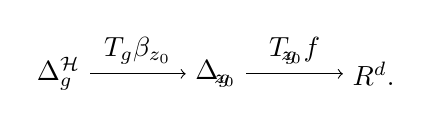
\begin{tikzpicture}[node distance=2cm, auto]
              \node (H) {$\Delta_g^{\mathcal{H}}$};
              \node (C) [right of=H] {$\Delta_{g \!\!\cdot\!\! z_0}$};
              \node (Rd) [right of=C] {$\Rd$.};
              \draw[->] (H) to node {$T_g\beta_{z_0}$} (C);
              \draw[->] (C) to node {$T_{g \!\!\cdot\!\! z_0}f$} (Rd);
            \end{tikzpicture}
            \end{center}
        Where $\beta_z(g) = g \cdot z \in \Conf$. This is a bijection.

        If we restrict this map to $T_gF|_{\Delta_g^{\mathcal{H}}}$
        this is equivalent to the Matrix $M(g \cdot z_0)$.
        Since $z_0$ takes at least 3 distinct values $M(g \cdot z_0)$
        is invertible for all $g \in \MSd$.
        
        The vector field $X_t(g)$ should give us a vector for every $g$ \st the snout
        follows $\gamma$:
            \[ M(g \cdot z_0) X_t(g) = \dot{\gamma}(t) . \]
        So $X_t(g) = M^{-1}(g \cdot z_0)\dot{\gamma}(t)$.
        
        Since $g(t)$ is the trajectory through $id$, we get that by construction
        $g(t) \cdot z_0$ is the unique horizontal lift of $\gamma$
        (see a text about initial value problems of ODEs).
    \end{proof}
\end{theorem}

\begin{remark}
    Note that there are cases where this differential equation does not have a solution
    for all $t$. This is discussed in \cite[Section 5]{Rodriguez07}.
\end{remark}


%%% Einträge im Glossar werden durch den Befehl
%%%    \glossar{begriff}{erklärung}
%%% vorgenommen.

\glossar{Gruppe}{Eine \emph{Gruppe} ist eine
Menge mit einer zweistelligen assoziativen Verknüpfung mit Einselement
und inversen Elementen.}

\glossar{Abelsche Gruppe}{Eine Gruppe
heißt \emph{abelsch}, wenn die Verknüpfung kommutativ ist.}

\glossar{Ä}{ein Eintrag, der mit einem Umlaut beginnt.}


\nocite{*}
\bibliography{lit}
%\printglossary
%\printindex
%\anhang

\end{document}
